\documentclass[a4paper]{article}

\usepackage[portuguese,english]{babel}
\usepackage[utf8]{inputenc}
\usepackage[T1]{fontenc}

\newcommand{\documentTitle}{Data Analysis and Transformation \\ TP1: Fundamentals of Signals and Systems}
\newcommand{\pdfTitle}{[ATD] TP1: Fundamentals of Signals and Systems}
\newcommand{\documentAuthors}{José Ribeiro (2008112181, jbaia@student.dei.uc.pt) \\ Pedro Magalhães (2009117002, pjrosa@student.dei.uc.pt)}

\title{\documentTitle}
\author{\documentAuthors}

\usepackage{hyperref}
\hypersetup{
	pdftitle = \pdfTitle
	,pdfauthor = \documentAuthors
	,pdfsubject = {Data Analysis and Transformation}
	,pdfkeywords = {Data Analysis and Transformation} {Signal Processing}
	,pdfborder = {0 0 0}
}

%\usepackage{subfig}
%\usepackage{amsmath}
%\usepackage{array}
\usepackage{anysize}
\usepackage{lscape}
\usepackage{amsmath}
\usepackage{graphicx}
\usepackage{caption}
\usepackage{amssymb}
%\usepackage[pdftex]{graphicx}
%\usepackage[table]{xcolor}

\hyphenation{}

\marginsize{3.0cm}{3.0cm}{3cm}{3cm}

\makeatletter

\begin{document}
\maketitle
\cleardoublepage

\tableofcontents
\cleardoublepage

\setlength{\parindent}{1cm}
\setlength{\parskip}{0.3cm}

\section{Introduction}
%%% TODO

\clearpage

\section{Exercise 1}
\subsection{Exercise 1.1}
Após a substituição das variáveis na expressão (assumindo $G\# = 25$), obtém-se a seguinte equação:
\begin{equation}
	x_{1}(t) = 2 \, sin(2 t) \, cos(11 t) + 5 \, cos^2 \, (8t)
	\label{eq:origsubst}
\end{equation}

\noindent Utilizando as identidades trigonométricas referidas em \emph{\nameref{subsubsec:trigident}}, procede-se agora à obtenção da expressão equivalente à equação $(\ref{eq:origsubst})$ segundo a forma
\begin{equation}
x_{1}(t) = \sum_{i} C_{i} \, cos(\omega_{i} t + \theta_{i})
\end{equation}

\subsubsection{Simplification}
\begin{eqnarray}
\label{eq:simplification}
x_{1}(t) & = & 2 \, sin(2 t) \, cos(11 t) + 5 \, cos^2 \, (8t) \\
	 & = & sin(2 t + 11 t) + sin(2 t - 11 t) + 5 \, cos^2 \, (8t) \\
	 & = & sin(13 t) + sin(- 9 t) + 5 \, cos^2 \, (8t) \\
	 & = & - cos\left(13 t + \frac{\pi}{2}\right) - cos\left(- 9 t + \frac{\pi}{2}\right) + 5 \, cos^2 \, (8t) \\
	 & = & cos\left(13 t + \frac{3 \pi}{2}\right) + cos\left(- 9 t + \frac{3 \pi}{2}\right) + 5 \, cos^2 \, (8t) \\
	 & = & cos\left(13 t + \frac{3 \pi}{2}\right) + cos\left(9 t + \frac{\pi}{2}\right) + 5 \, cos^2 \, (8t) \\
	 & = & cos\left(13 t + \frac{3 \pi}{2}\right) + cos\left(9 t + \frac{\pi}{2}\right) + 5 \left(\frac{1 + cos(2 * 8 t)}{2}\right) \\
	 & = & cos\left(13 t + \frac{3 \pi}{2}\right) + cos\left(9 t + \frac{\pi}{2}\right) + \frac{5}{2} \, cos(0) + \frac{5}{2} \, cos(16 t) \\
	 & = & \frac{5}{2} \, cos(0) + cos\left(9 t + \frac{\pi}{2}\right) + cos\left(13 t + \frac{3 \pi}{2}\right) + \frac{5}{2} \, cos(16 t)
\end{eqnarray}

\subsubsection{Trigonometric identities}
\label{subsubsec:trigident}
A simplicação faz uso das seguintes igualdades\footnote{Entre parênteses encontram-se os números dos passos entre os quais foram utilizadas.}:
\begin{equation}
sin(\theta) \, cos(\varphi) = \frac{cos(\theta - \varphi) + cos(\theta + \varphi)}{2}
\tag{3 to 4}
\label{eqnarr:trigident}
\end{equation}

\begin{equation}
cos(\theta + \frac{\pi}{2}) = -sin(\theta)
\tag{5 to 6}
\end{equation}

\begin{equation}
cos(\theta + \pi) = -cos(\theta)
\tag{6 to 7}
\end{equation}

\begin{equation}
cos(-\theta) = cos(\theta)
\tag{7 to 8}
\end{equation}

\begin{equation}
cos^2(\theta) = \frac{1 + cos(2 \theta)}{2}
\tag{8 to 9}
\end{equation}

\subsubsection{"Proof" of equality}
\noindent De forma a verificar que nenhum erro havia sido cometido durante a transformação da equação do sinal, um gráfico com a representação segundo as duas fórmulas foi gerado. A fórmula original encontra-se representada a azul; a tracejado vermelho encontra-se sobreposta a representação segundo um somatório de co-senos, segundo a fórmula obtida em \emph{\nameref{eq:simplification}}.

\begin{center}
	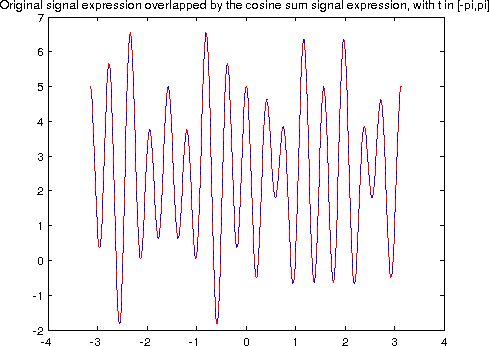
\includegraphics[scale=0.75]{images/ex11.png}
	\captionof{figure}{Original signal expression overlapped by the cosine sum signal expression, with $t \in [-\pi,\pi]$.}
	\label{fig:ex11}
\end{center}

\noindent Como é possível observar na figura \ref{fig:ex11}, a sobreposição das representações é perfeita.

\subsection{Exercise 1.2}
Fazendo uma simples substituição de $t$ por $n \, T_{s}$ na expressão obtida na alínea anterior obtém-se:
\begin{equation}
	x_{1}[n] = x_{1}(t) |_{t = n \, T_{s}} = \frac{5}{2} \, cos(0) + cos\left(9 \, n \, T_{s} + \frac{\pi}{2}\right) + cos\left(13 \, n \, T_{s} + \frac{3 \pi}{2}\right) + \frac{5}{2} \, cos(16 \, n \, T_{s})
\end{equation}

\subsection{Exercise 1.3}
O gráfico seguinte representa o sinal $x_1{1}(t)$ (a azul), para $t \in [-\pi, \pi]$ (com 500 elementos), sobreposto com o sinal $x_1{1}[n]$ (a vermelho) no mesmo intervalo, com um período de amostragem $T_ {s} = 0.1s$.

\begin{center}
	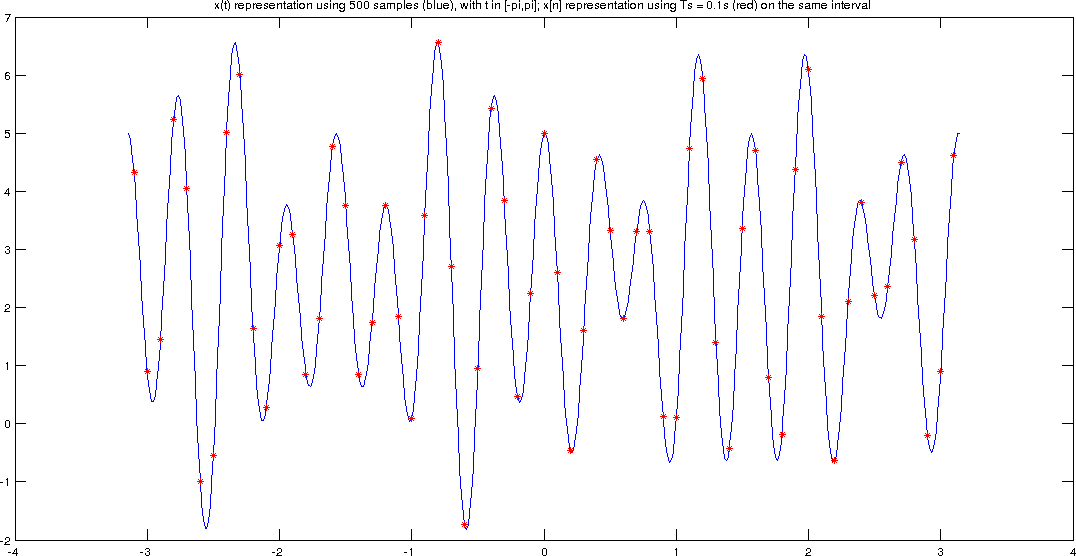
\includegraphics[scale=0.45]{images/ex13.png}
	\captionof{figure}{$x_1{1}(t)$ (blue), for $t \in [-\pi, \pi]$ (using 500 samples); $x_1{1}[n]$ (red) in the same interval, using $T_ {s} = 0.1s$.}
	\label{fig:ex13}
\end{center}

\noindent Como é possível observar na figura \ref{fig:ex13}, algumas amostras obtidas em $x_1{1}[n]$ apresentam um ligeiro desvio quando comparadas com o traçado do sinal $x_1{1}[n]$. Após alguma análise (incluíndo a soma das diferenças), concluímos que esse desvio se deve exclusivamente à perda de precisão decimal durante a criação do \emph{array} de espaçamento linear utilizado para o cálculo de $x_{1}(t)$.

\subsection{Exercise 1.4}
\noindent A energia de um sinal de tempo contínuo é dada, em $J$ (\emph{joules}), pelo integral do quadrado do seu módulo, isto é:
\begin{equation}
E = \int_{-\infty}^{\infty} |x(t)|^2 \, \mathrm{d} t
\end{equation}

\subsubsection{\texttt{MATLAB}'s \texttt{Symbolic Math Toolbox}}
\noindent Utilizando as funções de cálculo matemático simbólico do \texttt{MATLAB}, foi possível obter o valor exacto da energia; neste caso, o valor é de $\frac{83 \, \pi}{4} J \approx 65.1880 J$.
% TODO Missing time measure (optional).

\subsubsection{Trapezoidal Rule}
\noindent A \emph{Regra do Trapézio} é uma técnica de integração numérica que aproxima um integral calculando a soma da área dos trapézios formados por pontos da função. A aproximação do integral segundo esta regra considerando $N$ intervalos igualmente espaçados é:
\begin{equation}
\int_{a}^{b} f(x) \, \mathrm{d} x \approx \frac{b-a}{2 \, N} (f(x_{1}) + 2 f(x_{2}) + 2 f(x_{3}) + ... + 2 f(x_{N}) + f(x_{N+1}))
\end{equation}

\noindent Como no enunciado nos é pedida uma aproximação com erro inferior a 0.001, devemos calcular o número de intervalos de forma a garantir essa condição. Existe um número $\xi$ entre $a$ e $b$ em que o erro obtido é dado pela fórmula\footnote{Fórmula do erro da aproximação do integral pela Regra do Trapézio deduzida por Atkinson em \emph{An Introduction to Numerical Analysis}, 1989, John Wiley \& Sons, ISBN 978-0-471-50023-0.}.
\begin{equation}
error = -\frac{(b - a)^3}{12 \, N^2} \, f''(\xi)
\end{equation}

\noindent Como é evidente pela fórmula, o erro em módulo\footnote{O valor de $error$ assume valor positivo ou negativo consoante o integral seja sub ou sobrestimado, respectivamente.} evolui proporcionalmente a $f''$. Como tal, é possível concluir que, para que seja possível calcular $N$ de forma a garantir que $error$ seja o erro máximo, será necessário calcular o valor de $\xi$ para o qual $f''$ assume o seu valor máximo. Doravante (por motivos de simplificação), iremos assumir que:
\begin{equation}
M \ge f''(\xi)
\end{equation}

\noindent Depois de encontrado $M$, e colocando a fórmula em ordem a $N$, obtém-se que:

\begin{equation}
N = \left\lceil \sqrt{\left| \frac{(b - a)^3}{12 \, max\_error} \, M \right|} \, \right\rceil
\end{equation}

O cálculo da energia do sinal $x_{1}(t)$ efectuado com a Regra do Trapézio obteve como resultado o valor de $65.1880 J$, utilizando um \emph{step} de $0.000499s$ (correspondente a $N = 12589$). O cálculo demorou, em média\footnote{Média de 30 iterações.}, $0.105080s$. Por comparação com o integral calculado por cálculo simbólico, o menor $N$ para o qual se obtém um erro inferior a $0.001$ é $5$.

\subsubsection{Simpson's Rule}
\noindent A \emph{Regra de Simpson} é outra técnica de integração numérica que aproxima um integral calculando a soma da área das parábolas. A aproximação do integral segundo esta regra, considerando $N$ intervalos igualmente espaçados (onde $N \in 2 \, \mathbb{Z})$ é:
\begin{equation}
\int_{a}^{b} f(x) \, \mathrm{d} x \approx \frac{b-a}{3 \, N} [f(x_{1}) + 4 f(x_{2}) + 2 f(x_{3}) + 4 f(x_{4}) + ... + 2 f(x_{N-2}) + 4 f(x_{N-1}) + f(x_{n})]
\end{equation}

\noindent Como no enunciado nos é pedida uma aproximação com erro inferior a 0.001, devemos calcular o número de intervalos de forma a garantir essa condição. Existe um número $\xi$ entre $a$ e $b$ em que o erro obtido é dado pela fórmula:
\begin{equation}
error = \frac{(b-a)^5}{180 \, N} \, f^{(IV)} (\xi)
\end{equation}

\noindent Como é evidente pela fórmula, o erro evolui proporcionalmente a $f^{IV}$. Como tal, é possível concluir que, para que seja possível calcular $N$ de forma a garantir que $error$ seja o erro máximo, será necessário calcular o valor de $\xi$ para o qual $f^{IV}$ assume o seu valor máximo. Iremos assumir que: 
\begin{equation}
M \ge f^{(IV)}
\end{equation}

\noindent Depois de obter o M, podemos colocar a fórmula em ordem N, obtém-se\footnote{Deverá somar-se 1 a $N$ caso $N$ seja ímpar, de forma a garantir que $N \in 2 \mathbb{Z}.$}:
\begin{equation}
N = \left\lceil \sqrt[4]{\left| \frac{(b - a)^5}{180 \, max\_error} \, M \right|} \right\rceil
\end{equation}

\noindent O cálculo da energia do sinal $x_{1}(t)$ efectuado com a Regra de Simpson obteve como resultado o valor de $65.1880J$, utilizando um \emph{step} de $0.008118s$ (correspondente a $N = 776$). O cálculo demorou, em média\footnote{Média de 30 iterações.}, $0.116167s$. Por comparação com o integral calculado por cálculo simbólico, o menor $N$ para o qual se obtém um erro inferior a $0.001$ é $10$.

\subsection{Exercise 1.5}
\noindent O cálculo da energia de um sinal discreto é dado pela fórmula:
\begin{equation}
E = \sum_{n = -\infty}^{\infty} | x[n] |^2
\end{equation}

\noindent Como tal, para calcular a energia de um sinal $x[n]$ para $n$ correspondente ao intervalo $[a, b]$, basta calcular o somatório de todos os valores do sinal no intervalo $n \in \left[ sgn\left(\frac{a}{T_{s}}\right) \, \left\lfloor \left| \frac{a}{T_{s}} \right| \right\rfloor, sgn\left(\frac{b}{T_{s}}\right) \, \left\lfloor \left| \frac{b}{T_{s}} \right| \right\rfloor \right]$\footnote{Esta fórmula garante que os valores do intervalo (que é $\subset \mathbb{Z}$), quando multiplicados por $T_{s}$, correspondem a valores contidos no intervalo original.}, onde $T_{s}$ é o período de amostragem.

\noindent Após a substituição no cálculo do intervalo, obtém-se que $n$ pertence ao intervalo $[-31, 31]$. O valor da energia de $x_1[n]$ obtido para $n \in [-31, 31]$ é de aproximadamente $656.6213J$.
\clearpage

\section{Exercise 2}
\subsection{Exercise 2.1}
\noindent O sinal de tempo discreto utilizado foi o seguinte:
\begin{equation}
x[n] = 1.5 \, cos[0.025 \, \pi \, n] (u[n + 40] - u[n - 40])
\end{equation}

Após a substituição das variáveis nas expressões (usando $G\# = 25$) obtêm-se as seguintes equações:
\begin{eqnarray}
	y_{1}[n] & = & 0.4 \, x[n - 1] + 0.6 \, x[n - 3] - 0.2 \, x[n - 4] \\
	y_{2}[n] & = & 1.2 \, x[2n - 4] \\
	y_{3}[n] & = & x[n - 2] \, x[n - 3] \\
	y_{4}[n] & = & (n - 2) \, x[n - 3]
\end{eqnarray}

\noindent Apresentam-se as representações dos mesmos sinais para o intervalo $-50 \leq n \leq 50$:

\begin{center}
	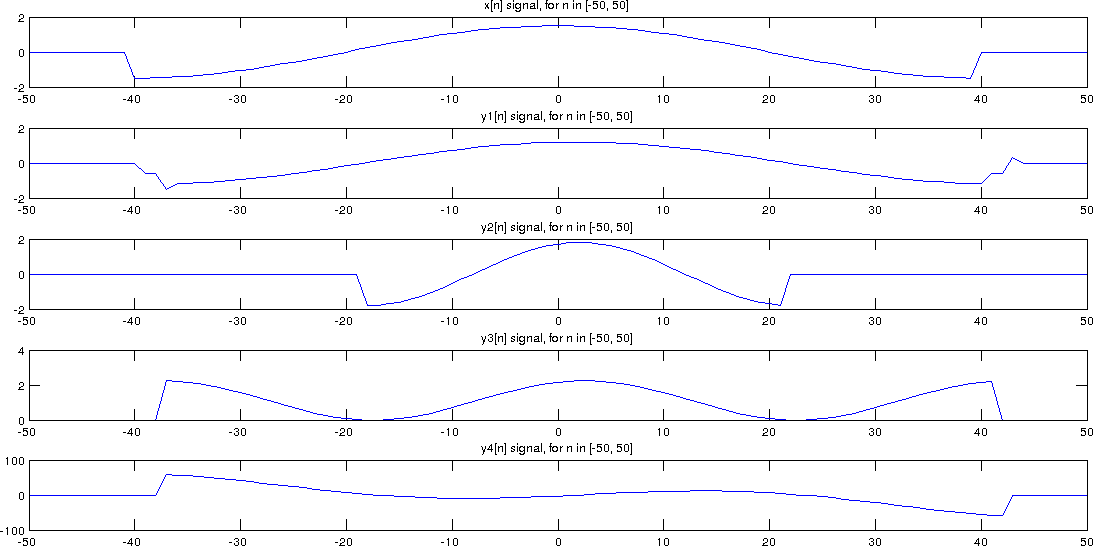
\includegraphics[scale=0.45]{images/ex21.png}
	\captionof{figure}{Top-down: $x[n]$, $y_{1}[n]$, $y_{2}[n]$, $y_{3}[n]$ and $y_{4}[n]$ plots, for $-50 \leq n \leq 50$.}
	\label{fig:ex21}
\end{center}

\subsection{Exercise 2.2}
\noindent Na imagem seguinte apresentam-se as entradas $x[n]$ e $x[n]$ com ruído uniforme no intervalo $]-0.2, 0.2[$ (em cima, a azul e vermelho, respectivamente) e a resposta do sistema $y_{1}[n]$ a essas mesmas entradas (em baixo, a azul a resposta à entrada $x[n]$, a vermelho a resposta à entrada de $x[n]$ com ruído).

\begin{center}
	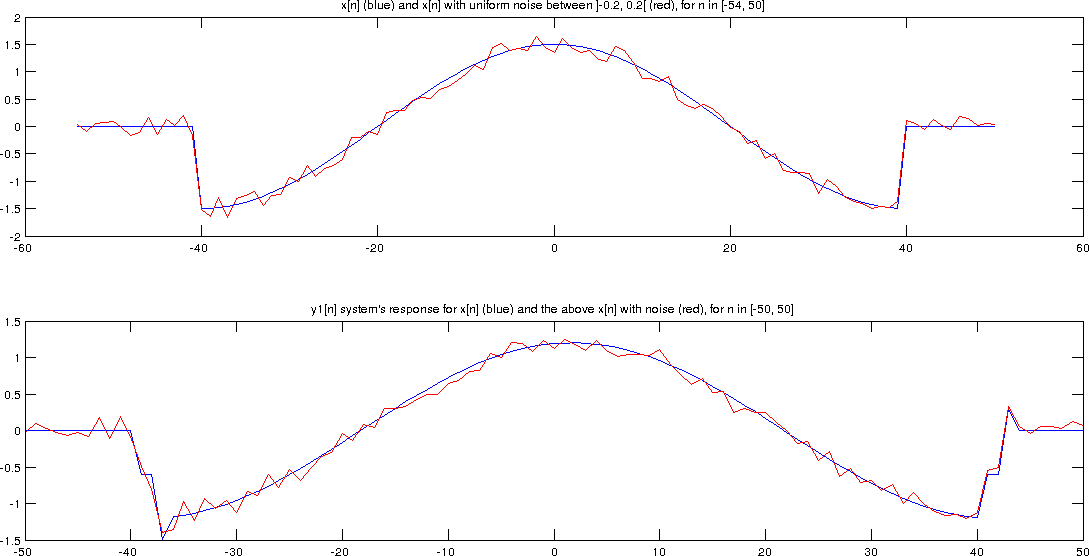
\includegraphics[scale=0.45]{images/ex22.png}
	\captionof{figure}{Above: $x[n]$ (blue) and $x[n]$ with uniform noise on the $[-0.2, 0.2]$; below: $y_{1}[n]$ response to $x_{1}[n]$ (blue) and $y_{1}[n]$ response to $x_{1}[n]$ with noise (red).}
	\label{fig:ex22}
\end{center}

\subsection{Exercise 2.3}
\noindent Para que um sistema seja linear, este deve verificar duas propriedades: \textbf{aditividade} e \textbf{homogeneidade}.

\noindent Para que um sistema verifique a propriedade de \textbf{aditividade}, é necessário que se verifique a seguinte igualdade:
\[
	\left\{
		\begin{aligned}
			T\{x_{1}[n]\} & = & y_{1}[n] \\
			T\{x_{2}[n]\} & = & y_{2}[n]
		\end{aligned}
	\right.
	\xrightarrow[\text{aditividade}]{}
	T\{x_{1}[n] + x_{2}[n]\} = y_{1}[n] + y_{2}[n]
\]

\noindent Para que um sistema verifique a propriedade de \textbf{homogeneidade}, é necessário que se verifique
\[
	T\{x[n]\} = y[n] \xrightarrow[\text{homogeneidade}]{} T\{a \, x[n]\} = a \, y[n]
\]

\noindent em que $a$ é uma constante arbitrária.

\noindent Em seguida analisa-se a linearidade dos sistemas $y_{1}[n]$, $y_{2}[n]$, $y_{3}[n]$ e $y_{4}[n]$.

\subsubsection{Análise de linearidade do sistema $\mathbf{y_{1}[n]}$}
\label{subsubsec:liny1}
\noindent \textbf{Aditividade}
\begin{eqnarray}
	T\{x_{1}[n]\}					& = & 0.4 \, x_{1}[n - 1] + 0.6 \, x_{1}[n - 3] - 0.2 \, x_{1}[n - 4] \\
	T\{x_{2}[n]\}					& = & 0.4 \, x_{2}[n - 1] + 0.6 \, x_{2}[n - 3] - 0.2 \, x_{2}[n - 4] \\
	\nonumber \\
	T\{x_{1}[n] + x_{2}[n]\}		& = & 0.4 \, (x_{1}[n - 1] + x_{2}[n - 1]) + 0.6 \, (x_{1}[n - 3] + x_{2}[n - 3]) \nonumber \\ && - 0.2 \, (x_{1}[n - 4] + x_{2}[n - 4]) \\
									& = & 0.4 \, x_{1}[n - 1] + 0.4 \, x_{2}[n - 1] + 0.6 \, x_{1}[n - 3] + 0.6 \, x_{2}[n - 3] \nonumber \\ && - 0.2 \, x_{1}[n - 4] - 0.2 x_{2}[n - 4] \\
	\nonumber \\
	T\{x_{1}[n]\} + T\{x_{2}[n]\}	& = & 0.4 \, x_{1}[n - 1] + 0.6 \, x_{1}[n - 3] - 0.2 \, x_{1}[n - 4] + 0.4 \, x_{2}[n - 1] + \nonumber \\ && 0.6 \, x_{2}[n - 3] - 0.2 \, x_{2}[n - 4]
\end{eqnarray}

\noindent Dado que $T\{x_{1}[n] + x_{2}[n]\} = T\{x_{1}[n]\} + T\{x_{2}[n]\}$, este sistema \textbf{verifica} a propriedade de \textbf{aditividade}. \\

\noindent \textbf{Homogeneidade}
\begin{eqnarray}
	T\{a \, x[n]\}					& = & 0.4 \, a \, x[n - 1] + 0.6 \, a \, x[n - 3] - 0.2 \, a \, x[n - 4] \\
									& = & a \, (0.4 \, x[n - 1] + 0.6 \, x[n - 3] - 0.2 \, x[n - 4])
\end{eqnarray}

\noindent Dado que $T\{a \, x[n]\} = a \, T\{x[n]\}$, este sistema \textbf{verifica} a propriedade de \textbf{homogeneidade}. Como verifica as duas condições, este sistema é \textbf{linear}.

\subsubsection{Análise de linearidade do sistema $\mathbf{y_{2}[n]}$}
\noindent \textbf{Aditividade}
\begin{eqnarray}
	T\{x_{1}[n]\}					& = & 1.2 \, x_{1}[2n - 4] \\
	T\{x_{2}[n]\}					& = & 1.2 \, x_{2}[2n - 4] \\
	\nonumber \\
	T\{x_{1}[n] + x_{2}[n]\}		& = & 1.2 \, (x_{1}[2n - 4] + x_{2}[2n - 4]) \\
									& = & 1.2 \, x_{1}[2n - 4] + 1.2 \, x_{2}[2n - 4] \\
	T\{x_{1}[n]\} + T\{x_{2}[n]\}	& = & 1.2 \, x_{1}[2n - 4] + 1.2 \, x_{2}[2n - 4]
\end{eqnarray}

\noindent Dado que $T\{x_{1}[n] + x_{2}[n]\} = T\{x_{1}[n]\} + T\{x_{2}[n]\}$, este sistema \textbf{verifica} a propriedade de \textbf{aditividade}. \\

\noindent \textbf{Homogeneidade}
\begin{eqnarray}
	T\{a \, x[n]\}					& = & 1.2 \, a \, x[2n - 4] \\
									& = & a \, (1.2 \, x[2n - 4])
\end{eqnarray}

\noindent Dado que $T\{a \, x[n]\} = a \, T\{x[n]\}$, este sistema \textbf{verifica} a propriedade de \textbf{homogeneidade}. Como verifica as duas condições, este sistema é \textbf{linear}.

\subsubsection{Análise de linearidade do sistema $\mathbf{y_{3}[n]}$}
\noindent \textbf{Aditividade}
\begin{eqnarray}
	T\{x_{1}[n]\}					& = & x_{1}[n - 2] \, x_{1}[n - 3] \\
	T\{x_{2}[n]\}					& = & x_{2}[n - 2] \, x_{2}[n - 3] \\
	\nonumber \\
	T\{x_{1}[n] + x_{2}[n]\}		& = & (x_{1}[n - 2] + x_{2}[n - 2]) (x_{1}[n - 3] + x_{2}[n - 3]) \\
									& = & x_{1}[n - 2] \, x_{1}[n - 3] + x_{1}[n - 2] \, x_{2}[n - 3] + \nonumber \\ && x_{2}[n - 2] \, x_{1}[n - 3] + x_{2}[n - 2] \, x_{2}[n - 3] \\
	T\{x_{1}[n]\} + T\{x_{2}[n]\}	& = & x_{1}[n - 2] \, x_{1}[n - 3] + x_{2}[n - 2] \, x_{2}[n - 3]
\end{eqnarray}

\noindent Dado que $T\{x_{1}[n] + x_{2}[n]\} \neq T\{x_{1}[n]\} + T\{x_{2}[n]\}$, este sistema \textbf{não verifica} a propriedade de \textbf{aditividade}; consequentemente, este sistema \textbf{não é linear}. \\
Procede-se ainda assim à análise da homogeneidade. \\

\noindent \textbf{Homogeneidade}
\begin{eqnarray}
	T\{a \, x[n]\}					& = & a \, x[n - 2] \, a \, x[n - 3] \\
									& = & a^2 (x[n - 2] \, a \, x[n - 3])
\end{eqnarray}

\noindent Dado que $T\{a \, x[n]\} \neq a \, T\{x[n]\}$, este sistema também \textbf{não verifica} a propriedade de \textbf{homogeneidade}.

\subsubsection{Análise de linearidade do sistema $\mathbf{y_{4}[n]}$}
\noindent \textbf{Aditividade}
\begin{eqnarray}
	T\{x_{1}[n]\}					& = & (n - 2) \, x_{1}[n - 3] \\
	T\{x_{2}[n]\}					& = & (n - 2) \, x_{2}[n - 3] \\
	\nonumber \\
	T\{x_{1}[n] + x_{2}[n]\}		& = & (n - 2) \, (x_{1}[n - 3] + x_{2}[n - 3]) \\
									& = & n \, x_{1}[n - 3] + n \, x_{2}[n - 3] - 2 \, x_{1}[n - 3] - 2 \, x_{2}[n - 3] \\
	T\{x_{1}[n]\} + T\{x_{2}[n]\}	& = & (n - 2) \, x_{1}[n - 3] + (n - 2) \, x_{2}[n - 3] \\
									& = & n \, x_{1}[n - 3] - 2 \, x_{1}[n - 3] + n \, x_{2}[n - 3] - 2 \, x_{2}[n - 3]
\end{eqnarray}

\noindent Dado que $T\{x_{1}[n] + x_{2}[n]\} = T\{x_{1}[n]\} + T\{x_{2}[n]\}$, este sistema \textbf{verifica} a propriedade de \textbf{aditividade}. \\

\noindent \textbf{Homogeneidade}
\begin{eqnarray}
	T\{a \, x[n]\}					& = & (n - 2) \, a \, x_{1}[n - 3] \\
									& = & a \, ((n - 2) \, x_{1}[n - 3])
\end{eqnarray}

\noindent Dado que $T\{a \, x[n]\} = a \, T\{x[n]\}$, este sistema \textbf{verifica} a propriedade de \textbf{homogeneidade}. Como verifica as duas condições, este sistema é \textbf{linear}.

\subsection{Exercise 2.4}
\noindent Para que um sistema seja invariante no tempo, é necessário que este verifique a seguinte propriedade:
\[
	T\{x[n]\} = y[n]
	\xrightarrow[\text{invariância no tempo}]{}
	T\{x[n - n_{0}]\} = y[n - n_{0}]
\]

Segue-se a análise da invariância no tempo dos 4 sinais.

\subsubsection{Análise de invariância no tempo do sistema $\mathbf{y_{1}[n]}$}
\begin{eqnarray}
	T\{x[n - n_{0}]\}	& = & 0.4 \, x[n - n_{0} - 1] + 0.6 \, x[n - n_{0} - 3] - 0.2 \, x[n - n_{0} - 4] \\
	y[n - n_ {0}]		& = & 0.4 \, x[n - n_{0} - 1] + 0.6 \, x[n - n_{0} - 3] - 0.2 \, x[n - n_{0} - 4]
\end{eqnarray}

\noindent Dado que $T\{x[n - n_{0}]\} = y[n - n_ {0}]$, pode-se concluir que o sistema \textbf{é invariante no tempo}. Dada a sua linearidade (verificada em \emph{\nameref{subsubsec:liny1}}), é possível concluir que este é um sistema \emph{SLIT}.

\subsubsection{Análise de invariância no tempo do sistema $\mathbf{y_{2}[n]}$}
\begin{eqnarray}
	T\{x[n - n_{0}]\}	& = & 1.2 \, x[2n - n_{0} - 4] \\
	y[n - n_ {0}]		& = & 1.2 \, x[2 \, (n - n_{0}) - 4] \\
						& = & 1.2 \, x[2 \, n - 2 \, n_{0} - 4]
\end{eqnarray}

\noindent Dado que $T\{x[n - n_{0}]\} \neq y[n - n_ {0}]$, pode-se concluir que o sistema \textbf{não é invariante no tempo}.

\subsubsection{Análise de invariância no tempo do sistema $\mathbf{y_{3}[n]}$}
\begin{eqnarray}
	T\{x[n - n_{0}]\}	& = & x[n - n_{0} - 2] \, x[n - n_{0} - 3] \\
	y[n - n_ {0}]		& = & x[n - n_{0} - 2] \, x[n - n_{0} - 3]
\end{eqnarray}

\noindent Dado que $T\{x[n - n_{0}]\} = y[n - n_ {0}]$, pode-se concluir que o sistema \textbf{é invariante no tempo}.

\subsubsection{Análise de invariância no tempo do sistema $\mathbf{y_{4}[n]}$}
\begin{eqnarray}
	T\{x[n - n_{0}]\}	& = & (n - 2) \, x[n - n_{0} - 3] \\
	y[n - n_ {0}]		& = & (n - n_{0} - 2) \, x[n - n_{0} - 3]
\end{eqnarray}

\noindent Dado que $T\{x[n - n_{0}]\} \neq y[n - n_ {0}]$, pode-se concluir que o sistema \textbf{não é invariante no tempo}.

\begin{center}
	NOTA: Foram apagados o .tex e os ficheiros de imagens relativos à fase final do relatório. Encontra-se apenas o .pdf relativo à versão final desse código, em report_final_version.pdf
\end{center}

\subsection{Exercise 2.5}
\noindent TODO % TODO

\subsection{Exercise 2.6}
\noindent TODO % TODO

\subsection{Exercise 2.7}
\noindent TODO % TODO

\section{Exercise 3}
\subsection{Exercise 3.1}
\noindent TODO % TODO

\subsection{Exercise 3.2}
\noindent TODO % TODO

\subsection{Exercise 3.3}
\noindent TODO % TODO

\subsection{Exercise 3.4}
\noindent TODO % TODO

\end{document}
